\chapter{Arquitetura de comércio eletrônico para a TV Digital} \label{cap:arquitetura-tcommerce}

Neste capítulo é apresentada uma arquitetura para provimento de comércio eletrônico
para o Sistema Brasileiro de TV Digital. A mesma é uma arquitetura distribuída, baseada em componentes
reutilizáveis, os \textit{Web Services}, conhecida como Arquitetura Orientada a Serviços.

\begin{comment}
Segundo \cite{sommerville2011soft}:

\begin{quote}
"sistemas grandes são sempre decompostos em sub-sistemas que fornecem algum conjunto de serviços relacionados.
Assim, o processo inicial de projeto consiste em identificar esses sub-sistemas e estabelecer um \textit{framework}
de controle e comunicação."
\end{quote}
\end{comment}

Desta forma, a arquitetura proposta foi definida, incluindo a implementação de um \textit{framework} de comunicação (baseado nos protocolos
HTTP e SOAP) que é apresentado sucintamente neste capítulo, e em mais detalhes no Capítulo \ref{cap:ncluasoap}.

\section{Requisitos da Arquitetura} \label{sec:req-arquitetura}

A arquitetura deverá atender aos requisitos apresentados na Tabela \ref{tab:requisitos-arquitetura} a seguir.

\begin{center}
	\begin{tabular}{|p{10cm}|c|c|}
	  \hline 
		\textbf{Requisito}& \textbf{Funcional} & \textbf{Não funcional} \\
		\hline 
		T-01) Estar preparada para adaptação em qualquer 
equipamento com qualquer implementação do \textit{middleware} Ginga, seja para dispositivos fixos (como conversores
digitais e TV's com conversores integrados), móveis (como \textit{Notebooks}) ou portáteis (como telefones celulares). & & x \\
		\hline 
		T-02) Utilizar, preferencialmente, serviços gratuitos da \textit{Web}. & & x \\
		\hline 
		T-03) Facilitar o desenvolvimento de aplicações interativas para o SBTVD, inclusive
		com relação ao tratamento de recursos de interface gráfica. & x & \\
		\hline 
		T-04) Tornar transparente para a aplicação de TVD os provedores de serviços utilizados,
		permitindo a substituição por outros apenas estendendo-se classes na aplicação cliente
		e implementando a comunicação SOAP/HTTP com os provedores desejados. & x &  \\
		\hline 
		T-05) Facilitar a extensão e a manutenção das aplicações com uso de orientação a objetos e padrões de projetos. & x &\\
		\hline 		
		T-06) Fazer interoperação com serviços de forma amigável a \textit{firewalls}. &  & x \\
		\hline 
		T-07) Integrar diferentes serviços para compor as funcionalidades a serem disponibilizadas aos usuários das aplicações de TVDi. & x &\\
		\hline 		
		\added{T-08) Ser compatível com padrões W3C e ABNT (Ginga-NCL)} &  & x \\
		\hline 		
	\end{tabular}
	\captionof{table}{Requisitos da Arquitetura de \textit{T-Commerce}}
	\label{tab:requisitos-arquitetura}
\end{center}


\section{Apresentação Geral} \label{sec:apresentacao-arquitetura}

A arquitetura proposta é baseada no conceito de \textit{Service Oriented Architecture} (SOA),
ou Arquitetura Orientada a Serviços\nomenclature{SOA}{\textit{Service Oriented Architecture}}, onde a aplicação
é construída de forma distribuída, utilizando diferentes \textit{Web Services}, podendo
haver diferentes provedores de serviços, que é o caso da proposta implementada.

Uma arquitetura de comércio eletrônico considera, comumente, o conceito de loja virtual, 
que precisa integrar diferentes serviços para prover as funcionalidades
necessárias aos usuários e ao gerenciamento da mesma. Em uma aplicação de \textit{T-Commerce}
não é diferente, o que muda é apenas a plataforma, tendo-se uma interface gráfica
de usuário específica para a TV Digital, considerando-se todas as questões
de usabilidade como uso de fontes maiores devido ao usuário
ficar afastado do aparelho de TV e de integração \textit{Web}-TV referentes a esta plataforma. 
Todos os serviços que a loja virtual já disponibiliza
precisam ser acessados pela interface de TV Digital. Desta forma, a arquitetura
orientada a serviços vem ao encontro dessa necessidade, permitindo a integração
de uma aplicação cliente em uma plataforma diferente, possuindo uma interface gráfica
para TV Digital, com os serviços já implementados pela loja.

SOA permite a integração de sistemas hetererogêneos por utilizar a tecnologia de \textit{Web Services} SOAP
que, diferentemente do modelo REST, define um contrato único que todos os provedores e consumidores
de serviços devem seguir (o protocolo SOAP), o que facilita a integração de tais sistemas.

\begin{comment}
Assim, para atender aos requisitos citados, a Figura \ref{fig:arquitetura-tcommerce} apresenta a arquitetura proposta.
Cada item da mesma é apresentado nas subseções a seguir, em que são representados os elementos de \textit{hardware}
ou provedores de serviço, bem como os elementos de \textit{software} (apenas os \textit{softwares} aplicativos são apresentados em tal figura). 
\end{comment}

Assim, para atender aos requisitos citados, a Figura \ref{fig:arquitetura-tcommerce} apresenta a arquitetura proposta.
Cada item da mesma é apresentado nas subseções a seguir, em que se adotam as seguintes convenções:
as letras representam os elementos de \textit{hardware}
ou provedores de serviço, e os números representam os elementos de \textit{software} (apenas os \textit{softwares} aplicativos são apresentados em tal figura). 


Adicionalmente, embora não constando da Figura \ref{fig:arquitetura-tcommerce} (para dar uma visão mais simples inicialmente), os seguintes \textit{softwares} são empregados (os quais são apresentados nos capítulos seguintes):
\begin{itemize}
	\item \textit{Framework} LuaOnTV 2.0;
	\item e \textit{Framework} de Comunicação de Dados.
\end{itemize}

\begin{center}
	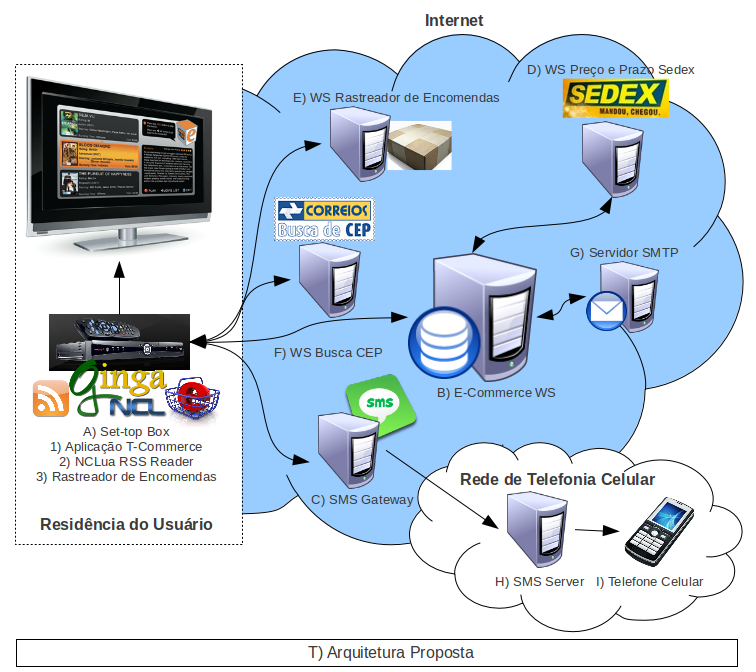
\includegraphics[width=0.8\textwidth]{TCommerce-Arquitetura.png}
	\captionof{figure}{Visão Geral da Arquitetura SOA proposta para \textit{T-Commerce}}
	\label{fig:arquitetura-tcommerce}
\end{center}

\subsubsection*{A) Conversor Digital/\textit{Set-top Box} (STB)\nomenclature{STB}{\textit{Set-top Box} (Conversor Digital)}}
Conversor digital, televisor com conversor integrado contendo o \textit{middleware} Ginga,
onde serão executadas as aplicações de TV Digital Interativa. Tais aplicações são conhecidas como
\textit{Thin Client} (Clientes Leves/Magros)\cite{sommerville2011soft} por apenas conterem uma camada de apresentação,
todas (ou grande parte) das regras de negócio são processadas no lado servidor.

Visando experimentos futuros, considera-se o uso de \textit{notebooks} ou telefones celulares com implementações
de Ginga-NCL para teste das aplicações desenvolvidas.

Tais equipamentos serão denominados daqui por diante como receptor/equipamento de TVD.

\subsubsection*{B) \textit{E-Commerce WS}} \label{sec:ecommercews}

\textit{Web Services} contendo as rotinas utilizadas em uma loja virtual convencional
na \textit{Internet}, que serão utilizadas pela aplicação de TV Digital para prover
comércio eletrônico pela TV. Tais \textit{Web Services} encapsulam todas as regras
de negócio para o gerencimento da loja virtual, como rotinas de cadastro de clientes,
produtos, pedidos, etc. A aplicação de TV Digital consumirá tal \textit{Web Service}
para prover muitas das funcionalidades disponíveis aos usuários.

\added{
O uso de tais \textit{Web Services} é essencial para centralizar
as regras de negócio utilizadas tanto pela aplicação de \textit{E-Commerce}
(normalmente acessada a partir de computadores ou dispositivos móveis como aparelhos celulares)
como pela aplicação de \textit{T-Commerce} (acessada a partir de receptores de TVD).
}

\subsubsection*{C) \textit{SMS Gateway}}

O \textit{Gateway} SMS\nomenclature{SMS}{\textit{Short Message Service}} é utilizado como intermediário para comunicação via SMS da loja com o cliente.
Devido à arquitetura proposta ser baseada em \textit{Web Services}, o uso do \textit{Gateway} facilita tal 
integração com a rede de telefonia celular.

Um serviço implementado na aplicação de \textit{T-Commerce} que requer o uso de SMS é a recuperação de senha, permitindo
que o usuário que esqueceu a senha, receba a mesma via mensagem SMS no telefone celular
que estiver cadastrado na loja. Tais serviços não são gratuitos e cobram por cada SMS enviado. 

O uso do \textit{Gateway} SMS é essencial por tornar transparente para a aplicação qual a operadora sendo utilizada
para enviar as mensagens SMS. Um das formas de envio de SMS é utilizando \textit{softwares} específicos para determinados
aparelhos celulares. No entanto, para automatizar tal processo seria necessário fazer a integração
com tal software por meio de alguma API, normalmente específica do \textit{software}. O uso
do \textit{Gateway} dispensa tal complexidade.

\subsubsection*{D) \textit{WS} Preço e Prazo Sedex}

Na arquitetura proposta, considerou-se que as entregas da loja
sejam feitas pela Empresa Brasileira de Correios e Telégrafos (ECT)\nomenclature{ECT}{Empresa Brasileira de Correios e Telégrafos},
denominada daqui em diante simplesmente como Correios. Desta forma, a obtenção de preços,
prazos de rastreamento das encomendas utiliza recursos dos Correios. \added{Desta forma,
o uso de um \textit{Web Service} dos Correios facilita a obtenção
de tais dados a partir de qualquer aplicação.}

\subsubsection*{E) \textit{WS} Rastreador de Encomendas}

Após o cliente ter decidido realizar a compra e finalizá-la, apesar
de já saber previamente qual a previsão para a entrega do produto,
um recurso muito utilizado é o rastreamento \textit{online} da encomenda.
Para tal funcionalidade, pelo fato de estarem sendo usados
os serviços de logística dos Correios, o rastreador
de encomendas para TV Digital realiza o rastreamento
\textit{online} de encomendas postadas por tal empresa. 

\subsubsection*{F) \textit{WS} Busca CEP}

A busca de endereço a partir de um Código de Endereçamento Postal (CEP)\nomenclature{CEP}{Código de Endereçamento Postal} 
é um requisito fundamental para
a aplicação de TVD, devido ao fato de o usuário
normalmente possuir apenas o controle remoto para entrada
de dados, utilizando o mesmo da mesma forma
como entra dados em um telefone celular.
Desta forma, a aplicação de \textit{T-Commerce} precisa
reduzir ao máximo a quantidade de dados que o usuário deve
digitar, para agilizar tal processo tedioso de entrada
de dados. Na arquitetura proposta foi utilizado um \textit{Web Service} para prover tal funcionalidade.

\subsubsection*{G) Servidor SMTP}

Como a aplicação de \textit{T-Commerce} possui recurso de recuperação de senha também por \textit{e-mail},
a arquitetura proposta inclui um servidor de \textit{Simple Mail Transfer Protocol} (SMTP).
Tal servidor é também conhecido como \textit{Mail Transfer Agent} (MTA)\nomenclature{MTA}{\textit{Mail Transfer Agent}},
que é responsável por transferir mensagens de correio eletrônico entre um computador e outro.
Por meio de tal servidor, a aplicação de TVD pode, por exemplo enviar a senha do usuário para seu \textit{e-mail}
ou confirmar a realização de uma compra.

\subsubsection*{H) SMS \textit{Server}}

Os \textit{Gateways} SMS fazem a integração com o SMS \textit{Server} de alguma(s) operadora(s)
para permitir o envio das mensagens SMS. 
Logo, o SMS \textit{Server} é o responsável direto pelo envio
das mensagens SMS pela rede de telefonia celular. Desta forma, o \textit{Gateway} apenas 
se encarrega de fazer a integração com o(s) servidor(es) de SMS, tornando tranparente para a aplicação
esta comunicação com o terminal celular do usuário.

\subsection{Casos de Uso das Funcionalidades da Arquitetura}

Para dar uma visão geral das funcionalidades providas pela arquitetura, tanto para os desenvolvedores
de aplicações de TV Digital Interativa (TVDi), quanto para os usuários finais, são apresentados os 
diagramas de casos de uso a seguir.


\begin{center}
	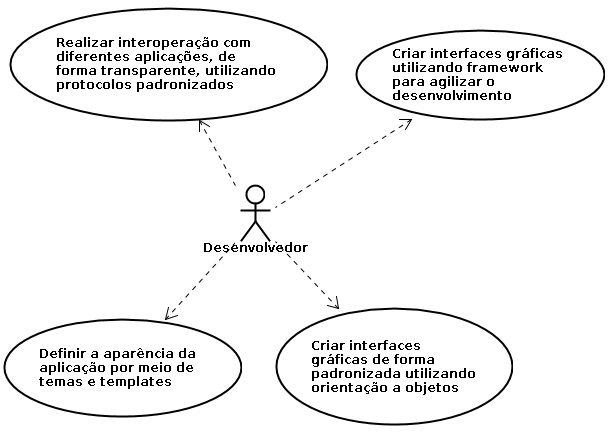
\includegraphics[width=0.7\textwidth]{TCommerce-Diagrama-Casos-de-Uso-Desenvolvedor.png}
	\captionof{figure}[Diagrama de Casos de Uso: Funcionalidades providas a desenvolvedores]{Diagrama de Casos de Uso das Funcionalidades providas a desenvolvedores de aplicações TVDi}
	\label{fig:use-case-developer}
\end{center}

A Figura \ref{fig:use-case-developer} apresenta as funcionalidades que a arquitetura provê aos desenvolvedores
de aplicações de TVDi, por meio dos \textit{frameworks} utilizados. Tais funcionalidades permitem
um grande aumento de produtividade no desenvolvimento de tais aplicações, reduzindo a quantidade
de código que os desenvolvedores precisam escrever e, consequentemente, o total de \textit{bugs}\footnote{Erro no funcionamento de um \textit{software}}.

\begin{center}
	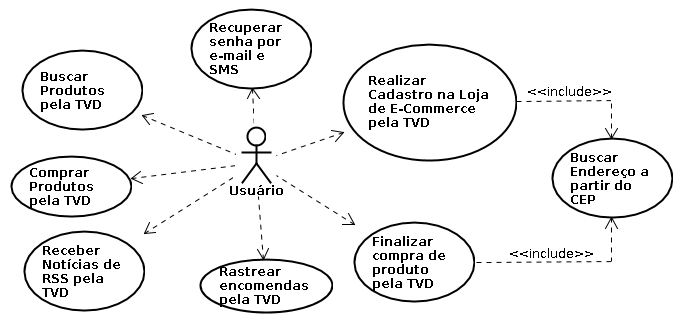
\includegraphics[width=0.7\textwidth]{TCommerce-Diagrama-Casos-de-Uso-Usuario.png}
	\captionof{figure}[Diagrama de Casos de Uso: Funcionalidades providas aos usuários]{Diagrama de Casos de Uso das Funcionalidades providas aos usuários das aplicações de TVDi desenvolvidas}
	\label{fig:use-case-usuario}
\end{center}

A Figura \ref{fig:use-case-usuario} apresenta as funcionalidades que a arquitetura provê aos usuários
de aplicações de TVDi. As funcionalidades implementadas são as consideradas mais comuns em sistemas
de \textit{E-Commerce} tradicionais.

\subsection{Tecnologias \textit{Core} da Arquitetura Proposta}

Em \cite{chu2007evolution} são tratadas as tecnologias \textit{core} para o provimento de comércio eletrônico,
divididas em quatro camadas: comunicação, apresentação e representação de informações, linguagens,
e armazenamento e recuperação de dados.

A camada de comunicação conta com as tecnologias necessárias para estabelecer a comunicação
entre as partes envolvidas nos sistemas de comércio eletrônico, assim como 
os protocolos utilizados para garantir a interoperabilidade entre as aplicações
que compõem tais sistemas. Utilizam-se, na arquitetura aqui proposta, as tecnologias
\textit{Hyper Text Transfer Protocol} (HTTP), \textit{Simple Object Access Protocol} (SOAP),
\textit{Simple Mail Transfer Protocol} (SMTP) e \textit{Short Message Service} (SMS).

A camada de apresentação e representação de informações contém as tecnologias
que definem o formato das informações, utilizado tanto para apresentação 
como para garantir a troca de informações entre sistemas heterogênos. 
Utilizam-se, na arquitetura aqui proposta, as tecnologias
\textit{eXtensible Markup Language} (XML), \textit{Really Simple Syndication} (RSS),
Lua, e imagens \textit{Joint Photographic Experts Group} (JPEG) e \textit{Portable Network Graphics} (PNG).

As linguagens de programação são utilizadas para a construção 
das regras de negócio das aplicações, definindo toda
a lógica das rotinas a serem executadas por elas.
São utilizadas as linguagens Java, \textit{Nested Context Language} (NCL) e Lua.

A camada de armazenamento e recuperação de dados
é responsável pelo armazenamento local ou remoto dos dados
das aplicações, como Sistemas Gerenciadores de Bancos de Dados (SGBD's).
São utilizadas as tecnologias MySQL \textit{DataBase Management System}, 
\textit{Java Database Connectivity} (JDBC) e \textit{Structured Query Language} (SQL).

\begin{center}
	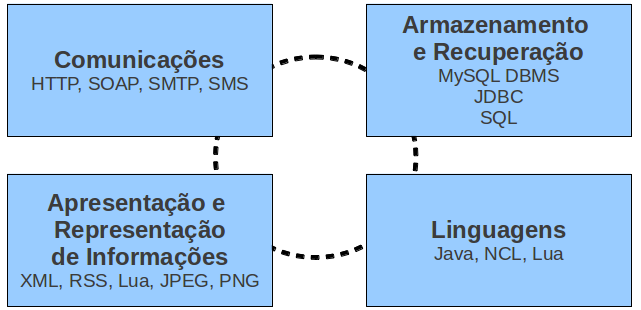
\includegraphics[width=0.8\textwidth]{TCommerce-Arquitetura-CoreTech.png}
	\captionof{figure}[Tecnologias \textit{Core} da arquitetura de \textit{T-Commerce}]{Tecnologias \textit{Core} da arquitetura de \textit{T-Commerce} (adaptada de \cite{chu2007evolution}).}
	\label{fig:tcommerce-core-tech}
\end{center}

A Figura \ref{fig:tcommerce-core-tech} apresenta as tecnologias empregadas na arquitetura proposta,
em cada uma das camadas supracitadas.


\section{Descrição dos Componentes de \textit{Software} da Arquitetura}

Conforme a Figura \ref{fig:arquitetura-tcommerce} exibida anteriormente,
nesta seção são apresentados os \textit{softwares} aplicativos que compõem
a arquitetura.

\subsection*{A) \textit{Set-top Box}}

\subsubsection*{A.1) Aplicação de \textit{T-Commerce}}

A aplicação é a interface gráfica pela qual o usuário pode realizar
compras por meio da TV Digital.

Os requisitos funcionais da aplicação foram baseados em avaliação
empírica das funcionalidades existentes na maioria dos sistemas de \textit{E-Commerce}
disponíveis no Brasil e amplamente conhecidos e utilizados.
A Tabela \ref{tab:app-tcommerce-requisitos} apresenta os requisitos funcionais e não funcionais atendidas pela aplicação.

\begin{center}
\scriptsize {
	\begin{tabular}{|p{11cm}|c|c|}
		\hline 
  		\textbf{Requisito} & \textbf{Funcional} & \textbf{Não Funcional} \\
		\hline
	  	A.1-01) Permitir a exibição de produtos em destaque ao iniciar a aplicação &  X &    \\
		\hline
		  A.1-02) Realizar a busca de produtos pelo título parcial &  X &    \\
		\hline
		  A.1-03) Adicionar produtos ao carrinho de compras &  X &    \\
		\hline
		  A.1-04) Remover produtos do carrinho de compras &  X &    \\
		\hline
		  A.1-05) Cadastrar vários endereços, permitindo ao usuário escolher um endereço
		   de entrega a partir da lista de endereços cadastrados &  X &    \\
		\hline
		  A.1-06) Permitir múltiplas formas de pagamento, possibilitando ao usuário selecionar uma das formas
		   suportadas &  X &    \\
		\hline
		  A.1-07) Cadastrar usuário &  X &    \\
		\hline
		  A.1-08) Realizar login de usuário utilizando \textit{e-mail} ou CPF &  X &    \\
		\hline
		  A.1-09) Buscar endereço a partir do CEP &  X &    \\
		\hline
		  A.1-10) Recuperar senha por \textit{e-mail} e SMS &  X &    \\
		\hline
		  A.1-11) Rastrear automatizadamente encomendas postadas pelos Correios,
		   exibindo ao usuário informações sempre que a situação
		   da encomenda mudar &  X &    \\
		\hline
		  A.1-12) Exibir preço e prazo de entrega, baseado em \textit{Web Services} dos Correios &  X &    \\
		\hline
		  A.1-13) Realizar processo de compra em etapas, permitindo que o usuário volte a uma etapa anterior,
		   antes de finalizar a compra, para alterar algum dado (como mudar a forma de pagamento) &  X &    \\
		\hline
		  A.1-14) Utilizar botões coloridos do controle remoto para o acionamento da maioria
		   das funções da aplicação &  X &    \\
		\hline
		  A.1-15) Processar grande parte das regras de negócio nos servidores \textit{Web} que integram a arquitetura,
		   desonerando o conversor digital da maior parte da carga de processamento, considerando
		   que o mesmo é um dispositivo de recursos restritos &   & X   \\
		\hline
		  A.1-16) Armazenar dos dados do carrinho de compras em memória RAM até a finalização da compra,
		   quando estes dados são enviados ao \textit{Web Service} para registro da mesma &   & X   \\
		\hline
		  A.1-17) Carregar dinâmicamente a lista de produtos a partir do \textit{Web Service} &   & X   \\
		\hline
		  A.1-18) Permitir a exibição de comunicados, ofertas de produtos e promoções & X &    \\
		\hline
	\end{tabular}
	\captionof{table}{Requisitos funcionais e não funcionais da aplicação de \textit{T-Commerce}}
	\label{tab:app-tcommerce-requisitos}
}
\end{center}

A aplicação é apenas um cliente que consome os \textit{Web Services} utilizados na arquitetura.
Assim, a maior parte da carga de processamento e regras de negócio é feita nos 
servidores \textit{Web} que hospedam os serviços. Quase todas as telas da aplicação
(que podemos chamar também de formulários ou páginas) fazem acesso a algum \textit{Web Service}
para obtenção ou registro de dados. Desta forma, a aplicação é totalmente dependente
de um canal de interatividade (também conhecido como canal de retorno)
para conexão à \textit{Internet} e acesso aos servidores \textit{Web} que hospedam os serviços.

Como o telespectador pode visualizar e comprar qualquer produto existente na loja,
e não somente aqueles que estejam em destaque, para a exibição dos produtos
sempre é feita uma consulta ao \textit{Web Service} de \textit{E-Commerce} da loja.
Em outros modelos de aplicação, como o apresentado em \cite{extra-vendas-tvd},
que exibem apenas os produtos em destaque, o telespectador não precisa
ter a TV conectada à \textit{Internet}, pois ele só visualiza os produtos 
enviados pela emissora, e não pode finalizar o processo de compra
pela TV. Desta forma, não há necessidade de conexão com a \textit{Internet}.
A arquitetura proposta vai além deste modelo, permitindo que o usuário possa comprar
qualquer produto e finalizar a compra direto da TV, o que exige a existência de um canal 
de interatividade.

A interface gráfica da aplicação foi desenvolvida
utilizando-se uma nova versão do \textit{framework} LuaOnTV\cite{junior2009luacomp}, cujas melhorias foram
desenvolvidas no presente trabalho de dissertação e são apresentadas em detalhes no Capítulo \ref{cap:luaontv}.
O LuaOnTV é a primeira e, até o momento em que esta dissertação foi desenvolvida,
a única biblioteca de componentes NCLua para criação de interfaces gráficas
em aplicações de TV Digital para o Ginga-NCL que se tem conhecimento.

Um \textit{screenshot}\footnote{Imagem capturada de uma tela de determinada aplicação em execução} da aplicação é apresentado na Figura \ref{fig:tcommerce-app-destaques}.
Tal figura mostra a tela inicial da aplicação, com os produtos em destaque na loja virtual (definidos no banco de dados da loja).
O usuário pode localizar um produto a partir de uma palavra contida no título,
inserindo tal valor por meio do controle remoto. 
O apêndice no final da dissertação mostra \textit{screenshots} de todas as telas da aplicação.

\begin{center}
	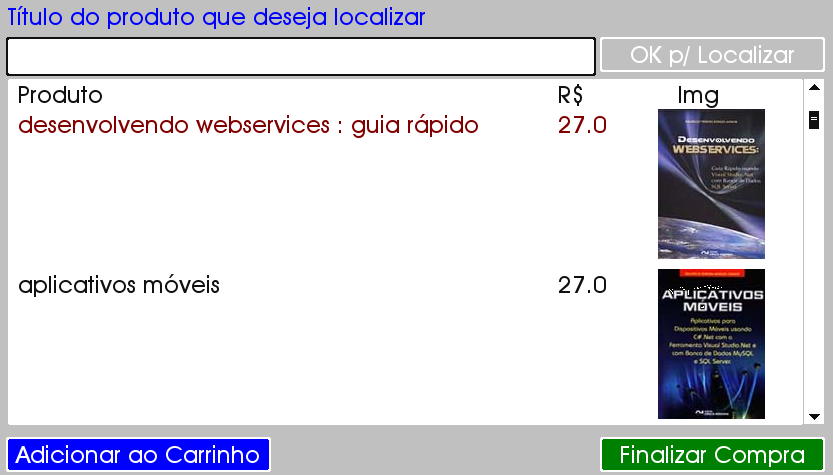
\includegraphics[width=0.8\textwidth]{CommerceApp/TCommerce-App-Destaques.png}
	\captionof{figure}{Aplicação de \textit{T-Commerce}: Tela inicial mostrando os produtos em destaque}
	\label{fig:tcommerce-app-destaques}
\end{center}

Toda a comunicação com os serviços que compõem a arquitetura é feita por meio do protocolo SOAP,
utilizando-se a implementação de SOAP para o Ginga-NCL denominada NCLua SOAP, construída
neste trabalho de dissertação e apresentada em detalhes no Capítulo \ref{cap:ncluasoap}. 

O processo de compra na aplicação de \textit{T-Commerce} desenvolvida é bastante simples e direto.
O diagrama de sequência apresentado na Figura \ref{fig:tcommerce-app-diagrama-seq-compra}
mostra como tal processo ocorre.

\begin{center}
	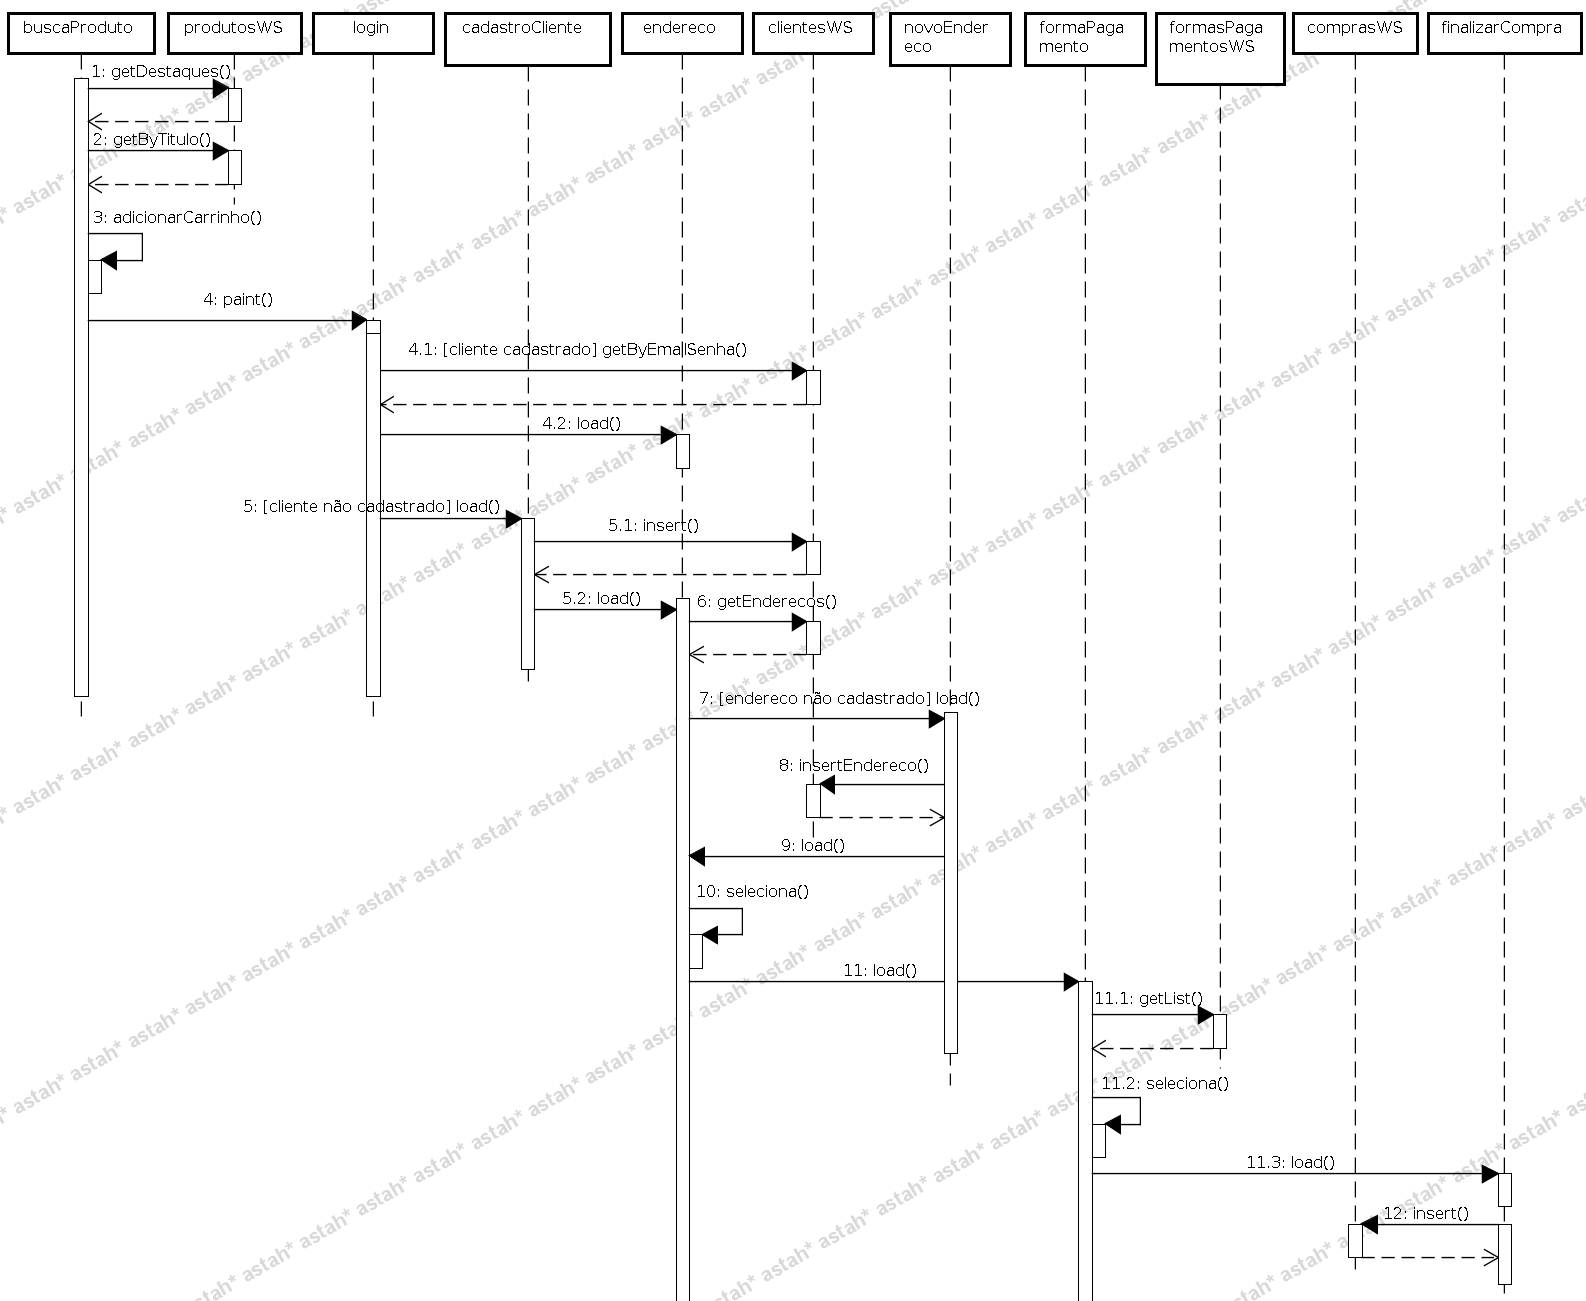
\includegraphics[width=1.2\textwidth]{TCommerce-Diagrama-Sequencia-Compra.png}
	\captionof{figure}{Aplicação de \textit{T-Commerce}: Diagrama de sequência do processo de compra}
	\label{fig:tcommerce-app-diagrama-seq-compra}
\end{center}

\subsubsection*{A.2) NCLua RSS \textit{Reader}}

Como pode ser visto na Figura \ref{fig:arquitetura-tcommerce}, o \textit{Set-top Box} 
(TV, notebook ou celular com o \textit{middleware} Ginga)
armazena a aplicação de \textit{T-Commerce} além de um leitor de RSS 
\nomenclature{RSS}{\textit{Really Simple Syndication}}desenvolvidos com as linguagens NCL e Lua.

Um arquivo RSS possui um formato XML e é utilizado para divulgação de notícias na \textit{Internet},
permitindo aos usuários assinarem os chamados \textit{feeds} RSS para
obterem as notícias de um determinado provedor desejado.
Os \textit{feeds} são os arquivos RSS que contêm as notícias em formato XML.
Com o RSS, a notícia vai até o usuário, no lugar de ele ir até a notícia.
Assim, tendo um leitor de RSS, o usuário pode adicionar vários \textit{feeds}
e receber várias notícias de diferentes provedores.

O leitor de RSS implementado para a TV Digital nesta dissertação é denominado 
\textit{NCLua RSS Reader}\footnote{\url{http://ncluarss.manoelcampos.com} e \url{http://labtvdi.unb.br}}.
Ele implementa o padrão RSS 2.0\cite{rss2} 
e compõe a arquitetura de \textit{T-Commerce} para permitir que, quando
o usuário não estiver acessando a aplicação da loja virtual pela TV, ele
possa ficar atualizado com as promoções que a loja esteja divulgando.

A aplicação utiliza o módulo LuaXML\footnote{\url{http://lua-users.org/wiki/LuaXml}} 
(que foi estendido para funcionar com Lua 5). Este é um parser XML escrito completamente
em Lua, que permite obter as notícias do \textit{feed} RSS e exibir em um equipamento de TVD.
A aplicação utiliza o módulo NCLua HTTP para fazer o \textit{download} do 
arquivo RSS diretamente do site do provedor de conteúdo, neste caso
o servidor \textit{Web} da loja virtual. O NCLua HTTP será apresentado no Capítulo \ref{cap:ncluasoap}.
O \textit{NCLua RSS Reader} ainda utiliza o módulo \textit{canvas} de NCLua para desenho 
da interface gráfica, além do módulo \textit{event} para tratamento de eventos.

A Figura \ref{fig:ncluarssreader} apresenta um \textit{screenshot} da aplicação de leitura de RSS em execução,
mostrando a mesma sendo exibida sobre o vídeo principal da emissora (em um ambiente
simulado, o \textit{Ginga Virtual Set-top Box}).

\begin{center}
	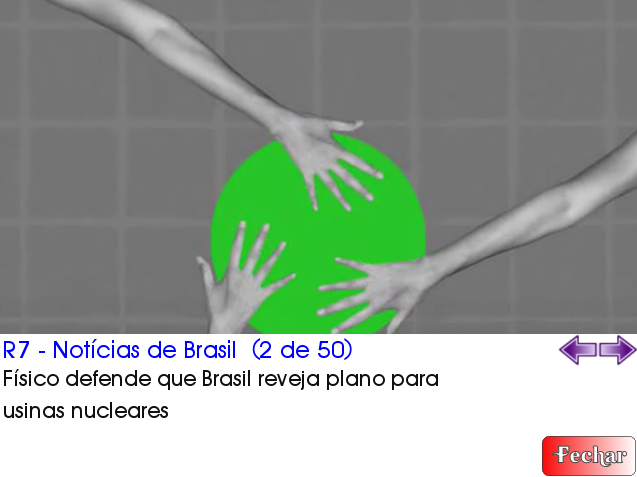
\includegraphics[width=1.00\textwidth]{nclua-rss-reader.png}
	\captionof{figure}{\textit{NCLua RSS Reader} - Leitor de Notícias para TV Digital}
	\label{fig:ncluarssreader}
\end{center}

\subsubsection*{A.3) Rastreador de Encomendas para TVD}

O rastreador de encomendas para a TV Digital faz acesso a este \textit{Web Service} desenvolvido
para o Ginga-NCL, utilizando as linguagens NCL e Lua e o módulo NCLua SOAP, este a ser apresentado no Capítulo \ref{cap:ncluasoap}.

As Figuras \ref{fig:rastreador-encomendas-tvd1} e \ref{fig:rastreador-encomendas-tvd2} apresentam \textit{screenshots} da aplicação em execução.
Tal aplicação, juntamente com o módulo NCLua SOAP, foi ganhadora do Concurso Latino-Americano de Conteúdo para TV Digital Interativa
\footnote{\url{http://clube.ncl.org.br/node/82}},
na categoria \textit{Widgets}, realizado pela PUC-Rio em 2010.

\begin{center}
	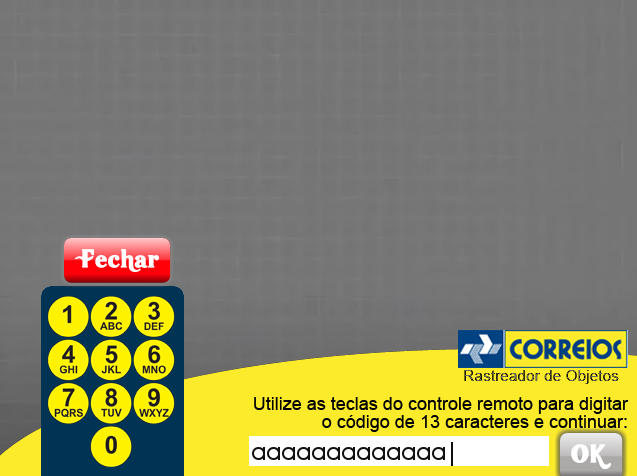
\includegraphics[width=0.9\textwidth]{rastreador/rastreador1.png}
	\captionof{figure}{Rastreamento de encomendas pela TVD: Inserção do código de rastreamento}
	\label{fig:rastreador-encomendas-tvd1}
\end{center}

\begin{center}
	
\includegraphics[width=0.9\textwidth]{rastreador/rastreador2.png}
	\captionof{figure}[Rastreamento de encomendas pela TVD: Situação da entrega da encomenda]{Rastreamento de encomendas pela TVD: Situação da entrega da encomenda (atualizada automaticamente a cada 5 minutos)}
	\label{fig:rastreador-encomendas-tvd2}
\end{center}

\subsection*{B) \textit{E-Commerce WS}}

O \textit{E-Commerce WS} contém um conjunto de \textit{Web Services} desenvolvidos utilizando-se o IDE NetBeans 6.7.1 e a  \textit{Java API for XML Web Services} (JAX-WS)
\nomenclature{JAX}{Java API \textit{for} XML}
\nomenclature{JAX-WS}{Java API \textit{for} XML \textit{Web Services}}
com o servidor de aplicações \textit{Glass Fish} 2.1 para execução dos \textit{Web Services}.
Tais ferramentas foram escolhidas por serem livres e multiplataforma,
amplamente utilizadas no mercado para o desenvolvimento de aplicações,
e pela familiaridade com as mesmas. O servidor de aplicações pode
ser qualquer outro (como \textit{Tomcat, Jetty ou JBoss}) que implemente a especificação de \textit{Servlet} 2.5.
Um \textit{Servlet} é uma classe Java \textit{server side}, ou seja, que executa
do lado do servidor \textit{Web}, sendo capaz de responder a requisições
HTTP com resposta em formato (X)HTML, XML e outros.
A escolha pelo \textit{Glass Fish} veio devido ao fato de ele ser a atual implementação
de referência para a plataforma \textit{Java Enterprise Edition} (Java EE)\nomenclature{Java EE}{\textit{Java Enterprise Edition}}, que provê as
tecnologias para desenvolvimento de aplicações \textit{Web} em Java.

Os métodos desenvolvidos em cada \textit{Web Service} foram implementados, baseado em um levantamento de requisitos
do que deve ter uma loja virtual, como já apresentado na Tabela \ref{tab:app-tcommerce-requisitos}. 
Utilizou-se a linguagem UML para modelar as classes e métodos
que comporiam os serviços.

A Figura \ref{fig:tcommerce-ws} apresenta um diagrama de classes com os \textit{Web Services}
implementados e seus respectivos métodos.

\begin{center}
	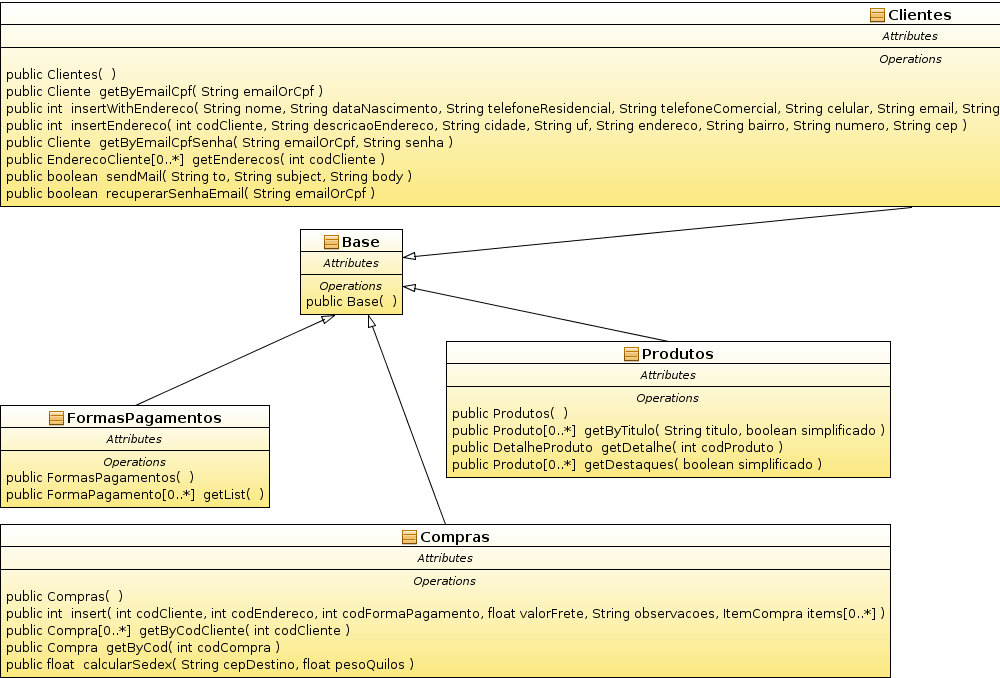
\includegraphics[width=1.00\textwidth]{TCommerce-ClassDiagramServices.png}
	\captionof{figure}{Diagrama de Classes dos \textit{Web Services} implementados}
	\label{fig:tcommerce-ws}
\end{center}

Cada \textit{Web Service} agrupa funcionalidades comuns. O "Clientes", por exemplo,
provê todas as funcionalidades para gerenciamento do cadastro do cliente, o "Compras",
todo o processo de compra, o "Produtos", todo o cadastro de produtos.

Estes \textit{Web Services} publicam os métodos a serem acessados pela aplicação de \textit{T-Commerce}.
Os mesmos são responsáveis pelo gerenciamento de todos os dados armazenados pela loja (como produtos, clientes
e pedidos de compra). Eles utilizam as classes Java apresentadas na Figura \ref{fig:tcommerce-ws-classes}
como base para seus métodos.

Tais classes são responsáveis pelo gerenciamento do cadastro do cliente, cadastro de produtos,
formas de pagamento, compras e tipo de frete. Para o armazenamento destes
dados foi utilizado o Sistema Gerenciador de Banco de Dados (SGBD) \textit{MySQL 5.1}
por ser um sistema multiplataforma, livre, bastante leve, que não requer
muitos recursos de hardware e amplamente utilizado no mercado, além
da familiaridade com o mesmo. No entanto, a arquitetura pode utilizar qualquer outro
banco de dados que for desejado, pois o acesso aos dados
é feito por meio da API \textit{Java Database Connectivity} (JDBC)\nomenclature{JDBC}{\textit{Java Database Connectivity}}
que é compatível com diversos SGBD's existentes no mercado. Além disto,
foi utilizado o padrão de projeto \textit{Data Access Objects} (DAO)\nomenclature{DAO}{\textit{Data Access Objects}}
que permite fazer uma separação total entre as classes de negócio e as instruções
SQL para acesso ao banco de dados.

\begin{center}
	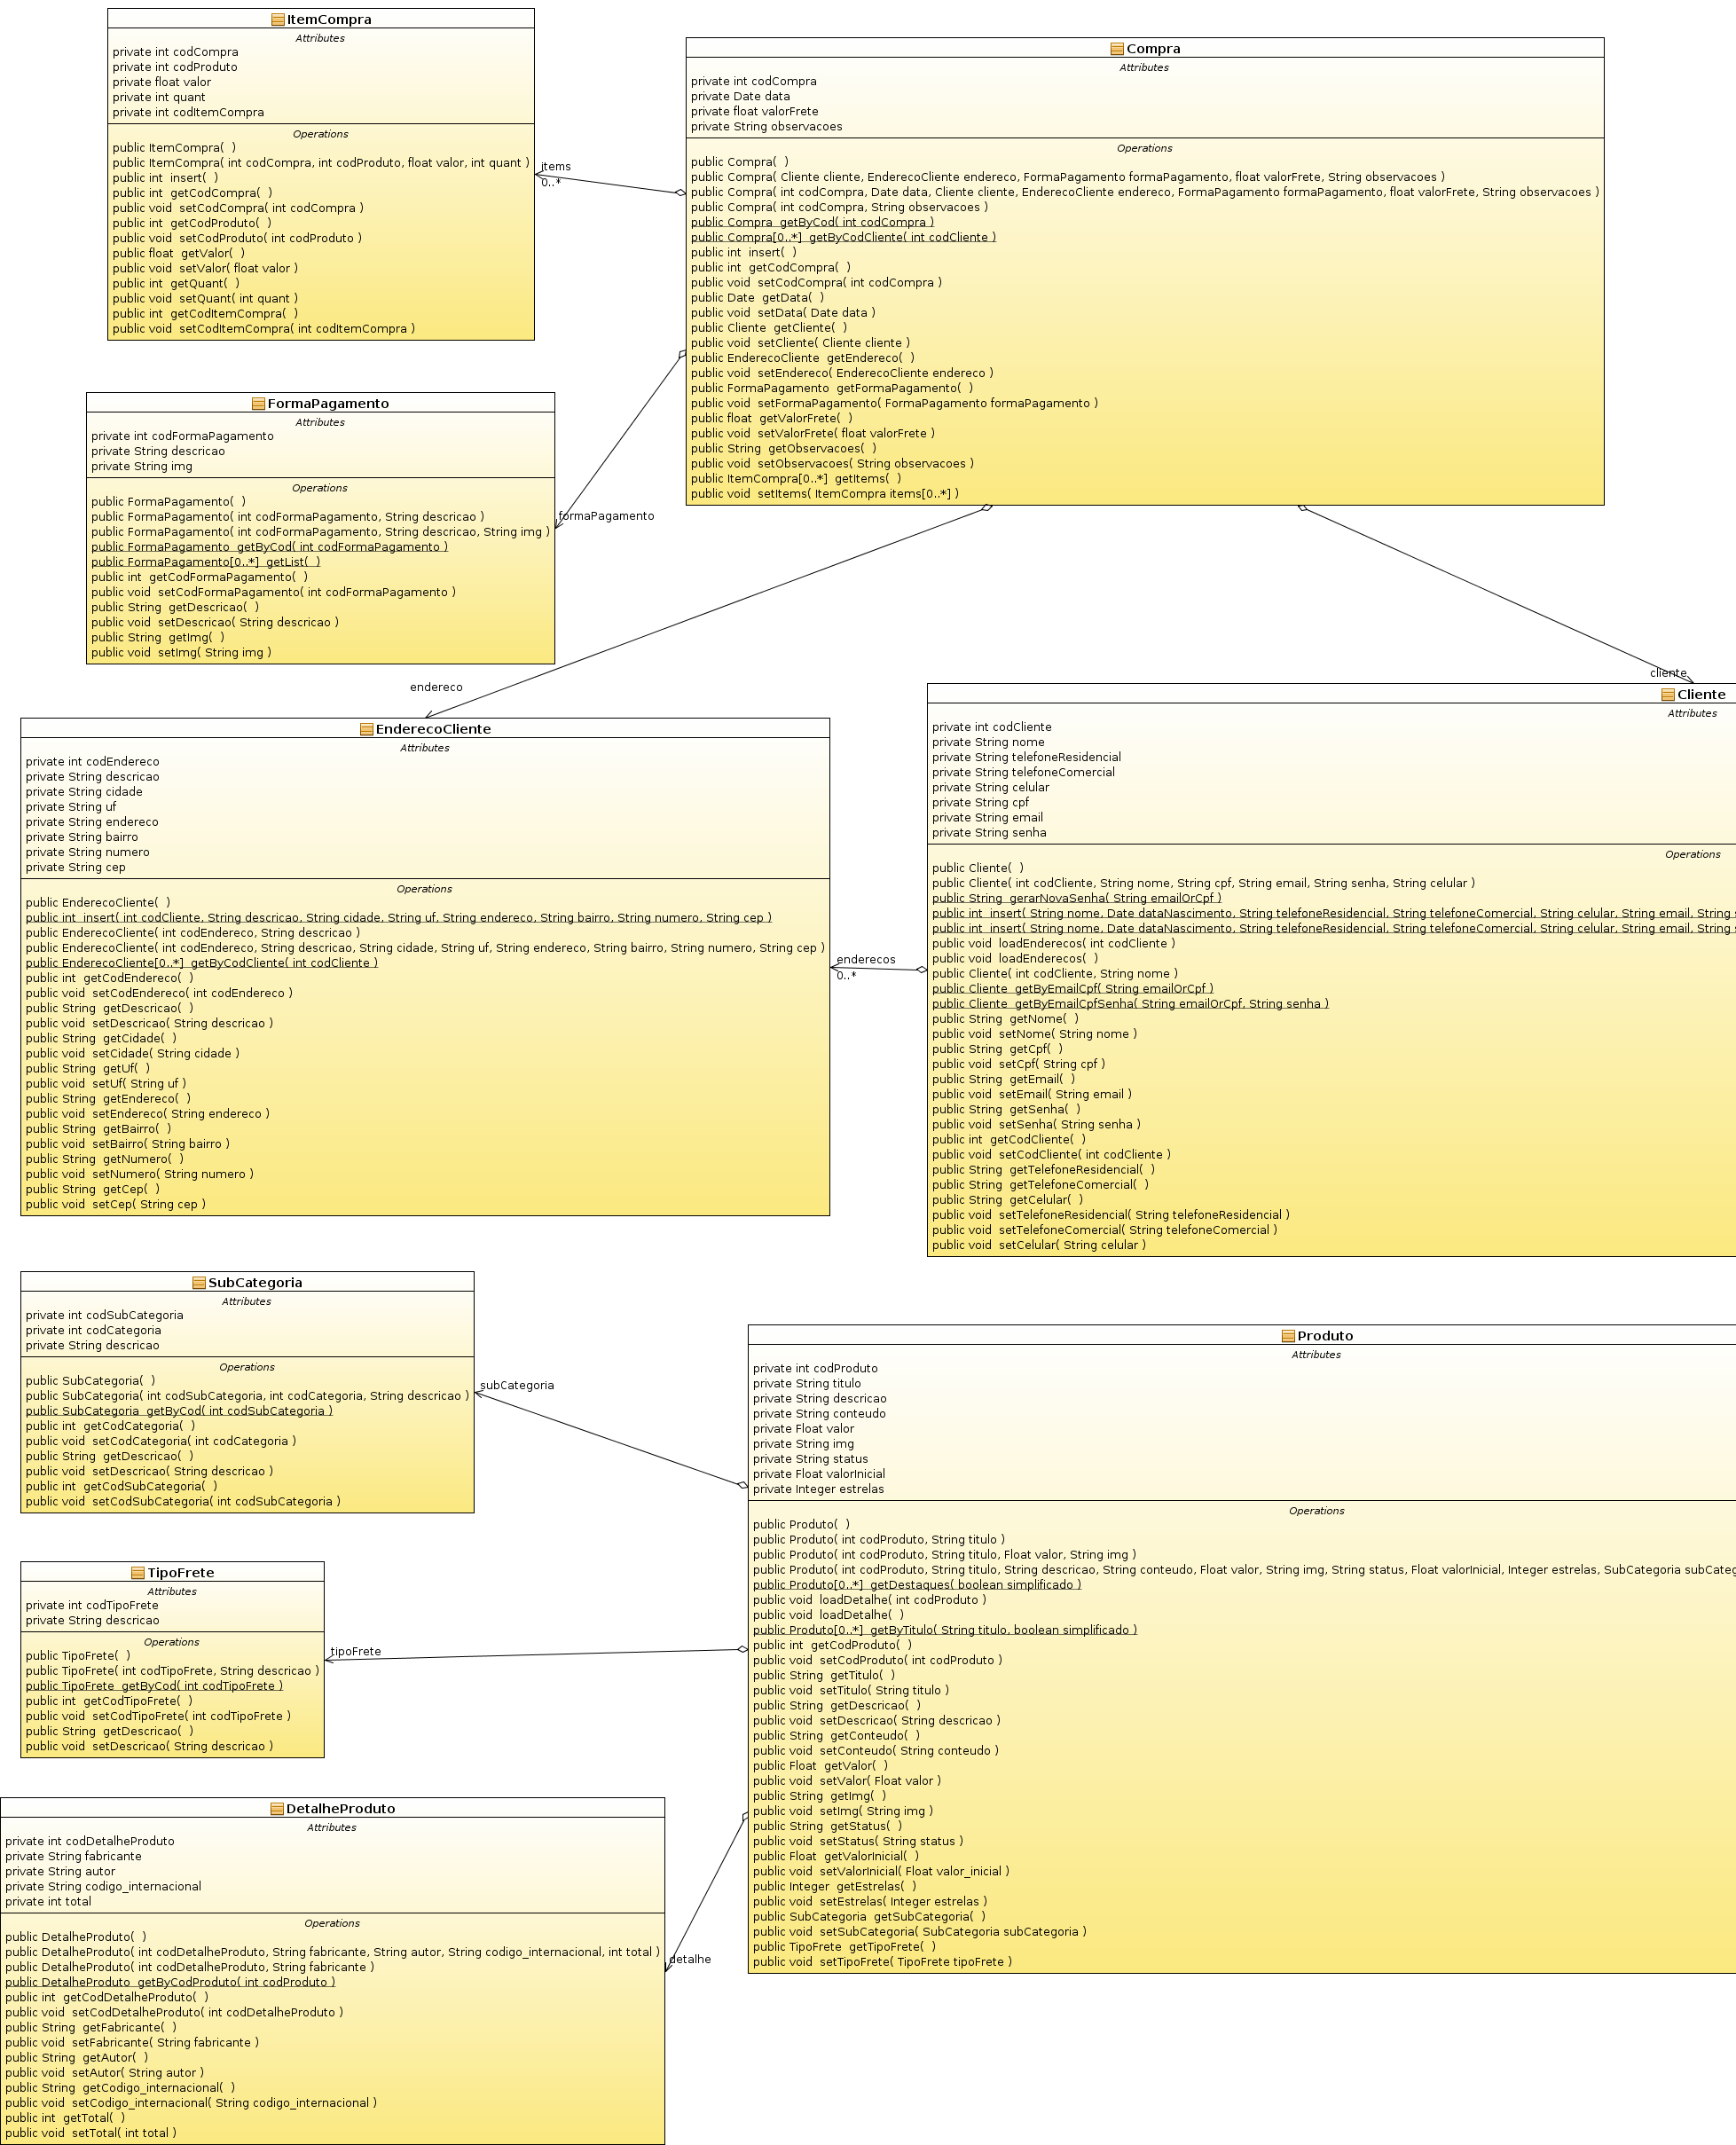
\includegraphics[scale=0.25]{TCommerce-ClassDiagramModel.png}
	\captionof{figure}{Diagrama das classes utilizadas internamente pelos WS's implementados}
	\label{fig:tcommerce-ws-classes}
\end{center}


Os \textit{Web Services} não utilizam nenhum \textit{framework} de persistência por falta
de familiaridade com tais tecnologias e restrições de tempo. No entanto,
a utilização de algum \textit{framework} como \textit{Hibernate} ou \textit{Java Persistent API} (JPA)\nomenclature{JPA}{\textit{Java Persistent API}}
não altera em nada a comunicação entre a aplicação de TVD e os \textit{Web Services}.
Tal mudança arquitetural pode ser feita para aumentar o nível de abstração
do acesso ao banco de dados e automatizar a geração das instruções
SQL\nomenclature{SQL}{\textit{Structured Query Language}} necessárias para isto, sob pena de aumentar o \textit{overhead} de acesso aos dados.

\subsection*{C) \textit{SMS Gateway}}

Para a arquitetura proposta, foi utilizado o \textit{Gateway} MyTalk\footnote{\url{http://www.mytalk.com.br}},
que permite o acesso via \textit{Web Services} SOAP. Contudo, tal componente
pode ser substituído na arquitetura por qualquer outro \textit{Gateway} SMS.
Todos os \textit{gateways} encontrados e testados, disponibilizam acesso via SOAP ou REST.
A escolha de tal serviço foi feita por ter sido o primeiro encontrado,
mas reitera-se que qualquer outro pode ser utilizado, levando-se em consideração
custo, resiliência, QoS (como tempo de resposta), etc.

Caso o usuário esqueça sua senha, ele pode informar seu \textit{e-mail} ou CPF na aplicação 
de TVD e recuperá-la via \textit{e-mail} ou SMS. Como ele normalmente estará na frente da TV, sair
deste local para ir até um computador e entrar no seu \textit{e-mail} para pegar 
uma nova senha é bastante incômodo. Como o celular é algo pessoal e
que geralmente as pessoas o mantêm por perto o tempo todo, o usuário
pode receber a nova senha sem precisar sair da frente da TV,
facilitando o processo de compra.

Neste caso, optou-se por a aplicação de TV enviar a requisição diretamente
ao \textit{Gateway} SMS, no lugar de requisitar ao \textit{Web Service} da loja (\textit{E-Commerce} WS)
para depois este despachar a requisição ao \textit{Gateway} SMS, 
no intuito de reduzir o tempo de resposta para a aplicação de \textit{T-Commerce}.
No entanto, esta abordagem tem a desvantagem de vincular a aplicação
a um determinado \textit{Gateway} SMS. Caso escolha-se utilizar
um \textit{Gateway} diferente, a aplicação precisará ser atualizada.
Centralizando tal regra de negócio no \textit{Web Service} da loja, não haverá
tal problema, mas aumentará o tempo de resposta da requisição
que precisará ser encaminhada ao \textit{Gateway}.

\subsection*{D) \textit{WS} Preço e Prazo Sedex}

Um dos recursos básicos que toda loja virtual deve prover a seus usuários é 
informar o preço e prazo para entrega do produto. Tals informações
podem ser decisivas para a concretização ou não da compra.

Os Correios são responsáveis por grande parte das entregas de produtos e correspondências em todo o país.
Desta forma, a arquitetura de \textit{T-Commerce} proposta faz integração com 
o \textit{Web Service} dos Correios\footnote{\url{http://www.correios.com.br/webservices/}} que permite calcular o preço e prazo de entrega
de uma correspondência/produto de/para qualquer lugar do país.
Logo, a aplicação de \textit{T-Commerce} consegue exibir o preço e prazo para entrega do(s) produto(s)
que o usuário deseja comprar, acessando tal \textit{Web Service}.

A atual versão da proposta permite apenas calcular preço e prazo de entrega de encomendas
utilizando o serviço de entregas rápidas dos Correios, denominado Sedex, mas
a obtenção de informações de entrega para outros serviços dos Correios
pode ser feita facilmente a partir da implementação atual.

A Figura \ref{fig:tcommerce-app-ws-correios} apresenta quais informações
podem ser obtidas do \textit{Web Service} dos Correios. 

\begin{center}
	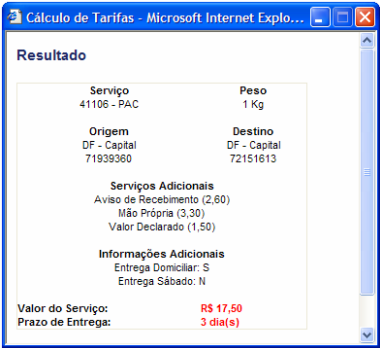
\includegraphics[width=0.8\textwidth]{TCommerce-PrecoPrazoSedex.png}
	\captionof{figure}[\textit{Web Service} dos Correios: Calculando preço e prazo de entrega de encomenda]{\textit{Web Service} dos Correios: Calculando preço e prazo de entrega de encomenda (fonte: \url{http://www.correios.com.br/webservices/}).}
	\label{fig:tcommerce-app-ws-correios}
\end{center}


O acesso ao serviço é feito a partir do \textit{E-Commerce WS} apresentado na Seção \ref{sec:ecommercews}.
Assim, a aplicação de \textit{T-Commerce} em NCLua envia uma requisição ao \textit{Web Service} "Compras"
que possui o método "calcularSedex" que retorna as informações sobre preço e prazo de entrega,
como apresentado no diagrama de classes da Figura \ref{fig:tcommerce-ws}.


\subsection*{E) \textit{WS} Rastreador de Encomendas}

Os Correios possuem um serviço na \textit{Internet} que permite ao usuário
saber a situação da entrega de uma determinada encomenda,
a partir do código de rastreamento da mesma.

No entanto, o usuário, para ficar atualizado da situação,
precisa periodicamente acessar tal página, gastando
tempo que ele poderia utilizar em outras atividades
mais importantes.

Assim, na arquitetura proposta, decidiu-se implementar um
serviço automatizado para rastreamento de encomendas,
onde o usuário possa acessar o serviço e deixar a tela
do mesmo aberta, sem precisar interagir com ela ou ficar voltando
lá para verificar se a situação da encomenda mudou.
Uma vez tendo aberta a tela do serviço, o usuário será
automaticamente notificado por meio de uma mensagem sonora,
que a situação da encomenda mudou.

O serviço está disponível via \textit{Web}\footnote{\url{http://rastreador.manoelcampos.com} e \url{http://labtvdi.unb.br}}
e foi também implementado em uma aplicação de TV Digital para o Ginga-NCL.

Como os Correios não disponibilizam
tal serviço de rastreamento por meio de um \textit{Web Service}, 
para facilitar a integração do serviço em diferentes arquiteturas, foi desenvolvido
um \textit{Web Service} para o rastreador. 
Este é responsável por fazer o \textit{parse} do código HTML da página do serviço dos Correios
e obter as informações sobre o rastreamento da encomenda. Tais informações
são extraídas e retornadas pelo \textit{Web Service} de forma estruturada, permitindo
a exibição delas facilmente em qualquer aplicação em diferentes plataformas.
Um exemplo é a aplicação iComenda\footnote{\url{http://itunes.apple.com/br/app/icomenda/id412358490?mt=8}}, 
desenvolvida por Maurício Júnior\footnote{\url{http://mauriciojunior.org}}, para os dispositivos
móveis iPhone, iPod e iPad, a partir do \textit{Web Service} disponibilizado.

\subsection*{F) \textit{WS} Busca CEP}

Infelizmente os Correios não disponibilizam um \textit{Web Service}
para a consulta de endereços a partir de um número de CEP.
Só há disponível uma página \textit{Web} para usuários finais\footnote{\url{http://www.buscacep.correios.com.br}}
que retorna os dados do endereço como uma imagem, para impedir (ou pelo menos dificultar bastante) 
que aplicações consigam acessar a página e extrair tais dados. Tal atitude provavelmente
é devida ao fato de os Correios terem um \textit{software} comercial, denominado
Guia Postal Brasileiro Eletrônico\footnote{\url{http://www.correios.com.br/servicos/cep/gpbe.cfm}}, 
contendo um banco de dados de CEP's, que é vendido na sua loja virtual e nas agências.

No entanto, existem alguns \textit{Web Services} de terceiros
que permitem obter o endereço a partir de um CEP. Qualquer
um deste serviços pode ser utilizado na arquitetura implementada
para permitir a obtenção de endereços.

Para a implementação realizada, foi escolhido o \textit{Web Service} disponível em 
\url{http://www.maniezo.com.br/webservice/soap-server.php}, por ter sido o primeiro
a ser encontrado. Tal serviço requer a realização de um cadastro prévio 
para poder acessá-lo, e com os poucos testes realizados, retornou os endereços
corretos e atualizados.

A aplicação de \textit{T-Commerce} faz acesso direto a tal serviço para obter um endereço,
utilizando-se o módulo NCLua SOAP.

\subsection*{G) Servidor SMTP}

Para envio de \textit{e-mail}, a aplicação de \textit{T-Commerce} acessa o método \textit{sendMail} do \textit{Web Service} "Clientes" do \textit{E-Commerce WS}, apresentado na Seção \ref{sec:ecommercews} e na Figura \ref{fig:tcommerce-ws}, para 
enviar \textit{e-mail} ao cliente. Desta forma, a aplicação cliente não acessa diretamente
o servidor de \textit{e-mail}. O \textit{E-Commerce WS} é que faz esta integração, despachando
a requisição para o servidor SMTP.

O \textit{E-Commerce WS} utiliza a API Java \textit{Mail}, funcionando como um cliente SMTP para
despachar a mensagem de \textit{e-mail}. Ele torna transparente para a aplicação, o servidor
de \textit{e-mail} utilizado e as configurações para acesso ao mesmo.

Na implementação feita, foi utilizado um servidor de \textit{e-mail} disponibilizado por um plano de hospedagem
profissional, logo é um serviço com custo mensal. No entanto, pode-se utilizar qualquer servidor de \textit{e-mail} que desejar,
como por exemplo um que seja disponibilizado por serviços de \textit{WebMail} gratuitos, amplamente
difundidos na \textit{Internet} e usados no cotidiano. 

\section{Diagrama de Distribuição/Implantação}

A Figura \ref{fig:diag-distribuicao} apresenta um diagrama de distribuição/implantação
que mostra como os componentes da arquitetura, apresentados na Seção \ref{sec:apresentacao-arquitetura} 
são distribuídos em diversos \textit{hardwares},
mostrando a arquitetura distribuída montada e a relação de dependência entre cada componente.
Tal diagrama apresenta todos os componentes de \textit{hardware} e \textit{software} da arquitetura proposta,
incluindo os \textit{softwares} aplicativos e os \textit{frameworks} implementados.

\begin{center}
	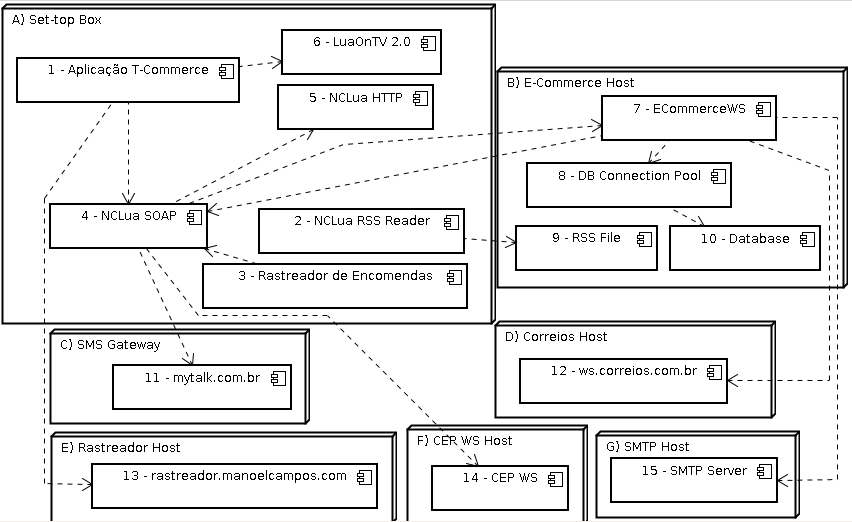
\includegraphics[width=1.00\textwidth]{TCommerce-Diagrama-Distribuicao.png}
	\captionof{figure}{Arquitetura de \textit{T-Commerce}: Diagrama de Distribuição/Implantação}
	\label{fig:diag-distribuicao}
\end{center}

As funcionalidades de cada componente são resumidas a seguir:

\begin{enumerate}[A)]
	\item \textit{Set-top Box} - Conversor de TV Digital, TV com conversor integrado, notebook ou celular que executa as aplicações de TVD desenvolvidas:
	\begin{itemize}
		\item 1 - Aplicação \textit{T-Commerce}: aplicação de comércio eletrônico para TVD (aplicação cliente);
		\item 2 - \textit{NCLua RSS Reader}: leitor de notícias para TVD, utilizado para ver notícias e ofertas de produtos;
		      da loja virtual;
		\item 3 - Rastreador de Encomendas para TVD: permite ao usuário rastrear a entrega do(s) produto(s) comprado(s) por meio da TV Digital,
		sendo notificado sempre que a situação da encomenda mudar;
		\item 4 - NCLua SOAP: módulo para acesso a \textit{Web Services} SOAP em aplicações NCLua para TVD;
		\item 5 - NCLua HTTP: módulo que implementa o protocolo HTTP, utilizado pelo NCLua SOAP e por aplicações
		          como o \textit{NCLua RSS Reader}. O módulo é apresentado no Capítulo \ref{cap:ncluasoap};
		\item 6 - LuaOnTV 2.0: \textit{framework} para construção da interface gráfica da aplicação de \textit{T-Commerce}.
	\end{itemize}
	\item \textit{E-Commerce Host} - Servidor \textit{Web} que hospeda os \textit{Web Services} a serem utilizados pela aplicação de \textit{T-Commerce}:
	\begin{itemize}
		\item 7 - \textit{ECommerceWS}: \textit{Web Services} da loja virtual, implementados em Java com a API JAX-WS;
		\item 8 - \textit{DB Connection Pool}: \textit{pool} de conexões ao banco de dados, implementado utilizando a API JDBC,
		que permite que conexões ao banco de dados sejam compartilhadas entre diferentes requisição ao \textit{Web Service},
		possibilitando um aumento de performance no acesso aos dados;
		\item 9 - \textit{RSS File}: arquivo RSS contendo as notícias e ofertas de produtos a serem divulgados pela loja virtual;
		\item 10 - \textit{Database}: banco de dados \textit{MySQL Server} 5.1 que armazena todos os dados da loja virtual, como cadastro
		de clientes, produtos e pedidos de compra.
	\end{itemize}
	\item SMS \textit{Gateway} - \textit{Gateway} para envio de mensagens SMS aos clientes:
	\begin{itemize}
		\item 11 - mytalk.com.br: \textit{Host} que hospeda o serviço \textit{MyTalk} SMS, um \textit{Gateway} para envio de mensagens SMS.
	\end{itemize}
	\item Correios \textit{Host} - \textit{Host} dos correios que hospeda \textit{Web Services} como os para consulta de preço e prazo de entrega de encomendas:
	\begin{itemize}
		\item 12 - ws.correios.com.br: \textit{Web Services} dos Correios para consulta de preço e prazo de entrega de encomendas.
	\end{itemize}
	\item Rastreador \textit{Host} - \textit{Host} que armazena o serviço de rastreamento de encomendas postadas pelos Correios:
	\begin{itemize}
		\item 13 - rastreador.manoelcampos.com: \textit{Web Service} de rastreamento de encomendas.
	\end{itemize}
	\item CEP WS \textit{Host} - \textit{Host} que hospeda um dos serviços de busca de endereço a partir do CEP:
	\begin{itemize}
		\item 14 - CEP WS: \textit{Web Service} maniezo.com.br que fornece o endereço a partir de um CEP
	\end{itemize}
	\item SMTP \textit{Host} - \textit{Host} que hospeda servidor de \textit{e-mail}:
	\begin{itemize}
		\item 15 - SMTP \textit{Server}: Servidor de \textit{e-mail} para envio de mensagens eletrônicas aos clientes da loja virtual.
	\end{itemize}
	\item SMS \textit{Server} - \textit{Host} de uma operadora de telefonia celular, responsável pela comunicação via SMS com o terminal celular do usuário.
\end{enumerate}


\section{Ambiente de desenvolvimento} \label{sec:dev-env}

Para o desenvolvimento do projeto foram utilizados:

\begin{itemize}
	\item sistema operacional GNU/Linux Ubuntu 10.10 como sistema \textit{desktop} para realização das tarefas de desenvolvimento;
	\item \textit{Astah Community} 6.1 (antigo \textit{Jude}) para modelagem UML;
  \item \textit{soapUI} 3.5.1 para testes de consumo de \textit{Web Services} SOAP;
	\item IDE\nomenclature{IDE}{\textit{Integrated Development Environment}} Eclipse 3.6 para desenvolvimento de aplicação Ginga-NCL:
	\begin{itemize}
		\item \textit{plugin} NCLEclipse 1.5.1;
		\item \textit{plugin} LuaEclipse 1.3.1;
	\end{itemize}
	\item ferramenta LuaDoc\footnote{\url{http://luadoc.luaforge.net}} para geração de documentação;
	\item implementação de referência do Ginga-NCL (Ginga Virtual Set-top Box 0.11.2);
	\item interpretador Lua para execução do \textit{scripts} fora do Ginga \textit{Virtual Set-top Box};	
	\item \textit{XVidCap} 1.1.7 para captura de \textit{screencasts}\footnote{Vídeo mostrando a execução de determinada aplicação} da aplicação em execução;
	\item IDE \textit{NetBeans} 6.7.1 para modelagem UML e desenvolvimento dos \textit{Web Services} da loja virtual, 
	utilizando API JAX-WS; servidor de aplicações \textit{Glass Fish} 2.1 para execução dos 
	\textit{Web Services} da loja virtual \footnote{\url{http://java.net/projects/openesb}};
	\item \textit{Java Development Kit} (JDK)\nomenclature{JDK}{\textit{Java Development Kit}} 1.6.0.24, o kit de desenvolvimento
	Java, contendo API's e ferramentas para desenvolvimento de aplicações;
	\item \textit{Java Runtime Environment} (JRE)\nomenclature{JRE}{\textit{Java Runtime Environment}} 1.6.0.24, o ambiente
	de execução Java para execução das aplicações Java como os \textit{Web Services} criados, os IDE's e outras
	ferramentas desenvolvidas em Java como o \textit{soapUI};
	\item \textit{MySQL Server} 5.1 como Sistema Gerenciador de Banco de Dados (SGBD)\nomenclature{SGBD}{Sistema Gerenciador de Banco de Dados} para os \textit{Web Services} da loja virtual;
	\item \textit{PhpMyAdmin} para administração do banco de dados;
	\item PHP 5.3 e Apache 2 para execução do \textit{PhpMyAdmin};
	\item \textit{VirtualBox} 4.0 e \textit{RemasterSys} para criação de distribuição Linux contendo todo o ambiente de desenvolvimento, com
	todas as ferramentas apresentadas acima.
\end{itemize}

\section[Distribuição GNU/Linux p/ desenvolvimento de aplicações]{Distribuição GNU/Linux para desenvolvimento, execução e teste de aplicações de TV Digital}

Com base no trabalho apresentado em \cite{soset}, foi gerada uma distribuição GNU/Linux
contendo todo o ambiente de desenvolvimento necessário para a construção das
aplicações apresentadas ao longo deste trabalho.
O ambiente contém todas as ferramentas apresentadas em \ref{sec:dev-env}. 
Tal distribuição GNU/Linux foi
elaborada com o intuito de facilitar a montagem do ambiente de desenvolvimento
necessário para a construção de aplicações NCL/Lua para a TV Digital.

A comunidade Ginga no Portal do Software Público disponibiliza
uma implementação de referência do sub-sistema Ginga-NCL em forma
de uma máquina virtual já com tal implementação compilada e instalada. 
Tal máquina virtual facilita bastante a montagem do ambiente
de desenvolvimento, uma vez que o processo de compilação
de tal implementação é bastante extenso, dependendo de diversos
softwares e bibliotecas, não sendo um processo trivial de 
ser executado, principalmente para usuários menos
experientes com distribuições GNU/Linux e ferramentas
de compilação de linha de comando. No entanto,
o uso de uma máquina virtual adiciona um \textit{overhead} 
de tempo no processo de teste das aplicações, uma vez
que os arquivos das mesmas precisam ser enviados via SSH para a máquina
virtual, apesar de tal processo ser automatizado com o \textit{plugin} NCL Eclipse.

Desta forma, a instalação da implementação de referência do Ginga-NCL diretamente no 
sistema operacional utilizado pelo desenvolvedor para as suas tarefas rotineiras
(como envio de \textit{e-mail's}, elaboração de documentos em \textit{suites} de escritórios, etc) 
e de desenvolvimento de sistemas agiliza bastante o processo de execução e teste
das aplicações interativas, pois, como o Ginga é instalado localmente na máquina real,
não há processo de transferência de arquivos para poder executar as aplicações.
Com isto, a execução das aplicações é praticamente instantânea, além de
obter-se melhor desempenho executando o Ginga nativamente no sistema 
operacional da máquina real, uma vez que o uso de uma máquina
virtual obviamente requer o consumo de mais memória RAM e processador
que executar o Ginga nativamente em uma máquina real.

A distribuição desenvolvida foi baseada na versão 10.10 do Ubuntu e permite
o uso do ambiente de desenvolvimento sem a necessidade de instalação do mesmo
na máquina do desenvolvedor, podendo ser dado \textit{boot} na máquina por meio
de um CD contendo tal distribuição, conhecido como \textit{Live CD}. Ela pode
ser instalada em uma máquina real, onde o usuário poderá utilizar tal
distribuição como seu sistema operacional \textit{Desktop} para
a realização de suas tarefas rotineiras e de desenvolvimento e ainda
pode ser instalada em uma máquina virtual, já com o ambiente gráfico e todas
as ferramentas de desenvolvimento necessárias.

A versão da implementação de referência do Ginga-NCL embarcada na distribuição
é a última (até a data de entrega de tal dissertação), a 0.11.2 revisão 23, disponível
na Comunidade Ginga do Portal do Software Público\footnote{\url{http://svn.softwarepublico.gov.br/trac/ginga/wiki/Building\_Wiki\_GingaNCL}}.

O processo de criação da distribuição GNU/Linux consistiu basicamente em:
\begin{itemize}
	\item instalar distribuição Ubuntu 10.10 em uma máquina virtual utilizando a ferramenta Virtual Box 4.0;
	\item baixar e compilar a implementação de referência do Ginga-NCL em tal máquina virtual, juntamente
	com todas suas dependêncais;
	\item instalar ferramentas de desenvolvimento e suas dependências (como JDK e JRE);
	\item configurar ferramentas de desenvolvimento para permitir a execução local de aplicações NCL/Lua;
	\item gerar uma nova distribuição a partir do ambiente criado, já com todas as ferramentas instaladas,
	utilizando o \textit{software} \textit{RemasterSys}\footnote{\url{http://remastersys.sourceforge.net}}.
\end{itemize}

Tal distribuição pode ser \replaced{obtida}{baixada} pelo \textit{site} do Laboratório de TV Digital Interativa da Universidade de Brasília\footnote{\url{http://labtvdi.unb.br}}.


